%!TEX encoding = utf-8 unicode
\documentclass[a4paper]{article}

\linespread{1.33}

\usepackage{kotex}
\usepackage{kotex-logo}
\usepackage[body={16cm,23cm}]{geometry}
\usepackage{fancyvrb}
\usepackage{minted}
\usepackage{setspace}
\usepackage{amsmath}
\usepackage{subfig}
\usepackage{graphicx}

\begin{document}
\title{Electric Experiment Report}
\author{조현종 201410935\and담당교수 김원준}
\date{2019 09 23}
\maketitle

\section{Abstract}
gradient 필터를 컨볼루션하여 magnitude와 phase 값을 구할수 있으며, 이를 통한 HOG 알고리즘을 간단하게 구현하여 인물을 구분할수 있을지 확인해본다.

\section{Experiment}
\subsection{Source code}

{\footnotesize
\begin{spacing}{1}
\begin{minted}[linenos=true, breaklines]{cpp}
#include <opencv2/imgproc.hpp>
#include <opencv2/highgui.hpp>
#include <math.h>
#include <iostream>
#include <stdlib.h>
#pragma warning(disable : 4996)

//define constant
#define PI 3.1416
#define CHANNEL 3
#define FILTER_H 3
#define FILTER_W 3

#define DEBUG_

//struct definition
struct pixel {
    float H;
    float W;
    float phase;
    float magnitude;
}typedef pixel;

using namespace cv;

//gradient filter definition
int filterX[9] = {
    -1, -1, -1,
    0,  0,  0,
    1,  1,  1
};
int filterY[9] = {
    -1, 0, 1,
    -1, 0, 1,
    -1, 0, 1
};

int main() {
    //open img
    Mat origImg = imread("ref6.jpg", cv::IMREAD_COLOR);
    int height = origImg.rows;
    int width = origImg.cols;
    
    //define iteration variable
    int i, j,h,w;
    
    Mat origImgGray = Mat::zeros(height, width, CV_8UC1);
    
    //conv. color to gray
    for (i = 0; i < height; i++) {
        //X
        for (j = 0; j < width; j++) {
            origImgGray.at<uchar>(i, j) = (origImg.at<Vec3b>(i, j)[0] + origImg.at<Vec3b>(i, j)[1] + origImg.at<Vec3b>(i, j)[2]) / 3;
        }
    }

    Mat outputImg(height, width, CV_8UC1);

    //allocation output pixel type
    pixel* output = (pixel*)calloc(height * width, sizeof(pixel));
    
    int max = INT_MIN, min = INT_MAX ;

    float comp;
    for (i = 0; i < height; i++) {
        //X
        for (j = 0; j < width; j++) {
            //convolution calculation
            for (h = 0; h < FILTER_H; h++) {
                for (w = 0; w < FILTER_W; w++) {
                    //countinue when outbound
                    if ((i - 1 + h < 0) || (i - 1 + h >= height)) continue;
                    if ((j - 1 + w < 0) || (j - 1 + w >= width)) continue;
                    //calc MAC gradient filter
                    output[i * width + j].W += (origImgGray.at<uchar>(i - 1 + h, j - 1 + w)) * (filterX[h * FILTER_W + w]);
                    output[i * width + j].H += (origImgGray.at<uchar>(i - 1 + h, j - 1 + w)) * (filterY[h * FILTER_W + w]);
                }
            }

            //calc phase
            output[i * width + j].phase = 180 * (atan2(output[i * width + j].H, output[i * width + j].W) / PI);
            if (output[i * width + j].phase < 0) {
                output[i * width + j].phase = output[i * width + j].phase + 180;
            }
            if (output[i * width + j].phase >= 180) {
                output[i * width + j].phase = 0;
            }

            //Phase quantization by 20 degree(unsigned)
            output[i * width + j].phase = (int)(output[i * width + j].phase / 20);

            //calc magnitude
            output[i * width + j].magnitude = sqrt(pow(output[i * width + j].W,2) + pow(output[i * width + j].H,2));
            
            //set max, min for normalize
            max = __max(output[i * width + j].magnitude, max);
            min = __min(output[i * width + j].magnitude, min);
        }
    }

    //magnitude normalize
    for (i = 0; i < height; i++) {
        for (j = 0; j < width; j++) {
            output[i * width + j].magnitude = 255 * (output[i * width + j].magnitude - min) / (max - min);
            outputImg.at<uchar>(i, j) = output[i * width + j].magnitude;
        }
    }

    int tileW = 16, tileH = 16, blkI, blkJ, sumBlk = 0;
    float block[15][7][9] = { 0, };

    //hog weight calc.
    for (i = 0; i <= height - tileH; i += 8) {
        for (j = 0; j <= width - tileW; j += 8) {
            blkI = i / 8;
            blkJ = j / 8;
#ifdef DEBUG
            std::cout << i << "," << j << std::endl;
#endif // DEBUG
            //calculation sum of demention's magnitude
            for (h = 0; h < tileH; h++){
                for (w = 0; w < tileW; w++) {
                    block[blkI][blkJ][((int)output[(h + i) * width + (w + j)].phase)] += 
                        output[(h+i)* width + (w+j)].magnitude;
                }
            }
            //sum of all block pixel's magnitude
            for (int k = 0; k<9; k++) {
                sumBlk += pow(block[blkI][blkJ][k],2) + 0.000001;
            }

            //calc. L-2 norm.
            for (int k = 0; k < 9; k++) {
                block[blkI][blkJ][k] = block[blkI][blkJ][k] / sqrt(sumBlk);
            }
            sumBlk = 0;
        }
    }
    //save hog weight
    FILE * file = fopen("output.csv", "w");
    fprintf(file, ",\n");
    for (i = 0; i <= height - tileH; i += 8) {
        for (j = 0; j <= width - tileW; j += 8) {
            blkI = i / 8;
            blkJ = j / 8;
            for (int k = 0; k < 9; k++) {
                fprintf(file, "%f,\n", block[blkI][blkJ][k]);
            }
        }
    }

#ifdef DEBUG
    for (i = 0; i < height; i++) {
        for (j = 0; j < width; j++) {
            std::cout << output[i * width + j].phase;
        }
        std::cout << std::endl;
    }
    //show result for debug
    imwrite("output.bmp", outputImg);
    imshow("orig", origImgGray);
    imshow("result", outputImg);
    waitKey(5000);
#endif // DEBUG
}

\end{minted}
\end{spacing}
}


\subsection{Result}
인풋 이미지 Figure~\ref{fig:refImg}에서, 각 이미지를 HOG weight로 변환 한뒤 ref.이미지와 각 compare 1, compare 2 이미지를 뺀 값을 그래프 Figure~\ref{fig:refSubGraph}로, 뺀값의 절대값을 구한 값을 그래프 Figure~\ref{fig:refSubABSGraph} 나타내었다. 파란색은 $reference - compare1$ 사람간을 비교한 값이며, 주황색은 $reference - compare2$ 사람과 풀을 비교한값이다.
\begin{figure}
    \centering
    \subfloat[reference]{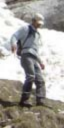
\includegraphics[]{ref.png}}
    \quad
    \centering
    \subfloat[compare 1]{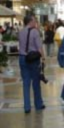
\includegraphics[]{compare1.png}}
    \quad
    \centering
    \subfloat[compare 2]{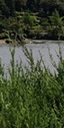
\includegraphics[]{compare2.png}}
    \caption{input으로 주어진 이미지}
\label{fig:refImg}
\end{figure}
\begin{figure}
    \begin{center}
        \fbox{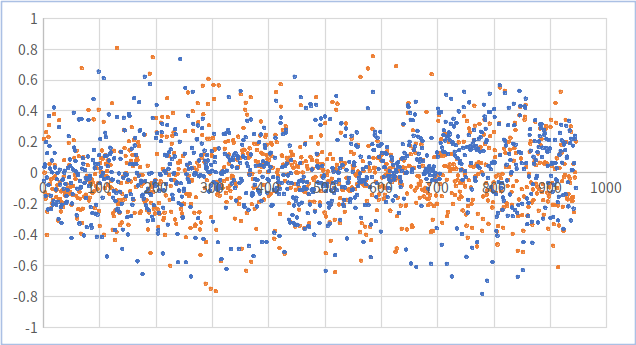
\includegraphics[width = 0.6 \linewidth]{ref-comp.png}}
        \caption{compare 1, 2와 Ref.와의 HOG weight 차 비교 그래프}
        \label{fig:refSubGraph}
    \end{center}
\end{figure}
\begin{figure}
    \begin{center}
        \fbox{\includegraphics[width = 0.6 \linewidth]{ref-compABS.eps}}
        \caption{compare 1, 2와 Ref.와의 HOG weight 차의 절대값 비교 그래프}
        \label{fig:refSubABSGraph}
    \end{center}
\end{figure}

\section{discussion}
본 코드는 gradient filter를 기반으로한 edgedetecting을 기본으로 하여, 각 픽셀의 magnitude와 radian을 기반으로 유사 hog 알고리즘 구현을 목표하였다. gradient filter란,\\
$x$ 매트릭스인 
$\begin{bmatrix} 
    -1 & -1 & -1 \\
    0 & 0 & 0 \\
    1 & 1 & 1 
\end{bmatrix}$
\quad
와, $y$ 매트릭스인
$\begin{bmatrix} 
    -1 & 0 & 1\\
    -1 & 0 & 1\\
    -1 & 0 & 1 
\end{bmatrix}$
\\이며, 이를 컨볼루션 하는 것으로 주변 상하, 좌우 픽셀과의 차를 구하고 두 좌표의 원점으로부터 길이를 구해 magnitude, $tan^{-1}()$하는것을 통해 radian을 구할수 있다. \\
HOG는 이미지를 일정 크기의 block으로 나눈뒤, radian을 기준으로 양자화해 블록별로 합산하는것으로 얻어진다. 위 코드에서는 128*64의 인풋 이미지를 입력받으며, 16*16의 블럭 사이즈, stride를 8, 양자화를 9단계로 설정하였다. 결과적으로 $(\frac{64}{8} - 1)\times(\frac{128}{8}-1)\times9=945$개의 결과가 나오게 되며, 이 값을 비교하면 이미지의 유사도를 판단할수 있다.\\
그래프~Figure\ref{fig:refSubGraph}를 보면 한눈에 두 이미지 compare 1, 2간의 차이가 보이지는 않는 편이다. 하지만, 각 값의 합이 0에 얼마나 가까운지를 보는것으로 각 값이 얼마나 유사한지를 확인할수 있다. 위 코드를 이용해 얻은 reference 이미지와 compare1 이미지 HOG weight의 총합은 7.7이며, compare 2 이미지와의 총합은 -20.5의 결과가 나와, 사람간의 비교가 0에 가까웠지만, 값들의 절대값들의 총합은 170과 166으로 오히려 사람과 사람을 비교했을때가 값이 높았다. \\
실제 이론과 결과를 비교하여 보았을때, 생각보다 명확한 차이가 나타난것 같지는 않았다. 몇가지 이유가 있을것으로 예상하였는데, 첫째로 기준이 되는 ref. 이미지에서 사람이 아닌 배경에도 엣지가 명확한 부분이 있어 기준 데이터로 삼기 어려웠을것이고, 두번째로 HOG 구현방식이 논문보다 축약된 방식이였으며, 세번째로 사람 여부의 분류를 weight의 학습을 통한 분류가 아닌 사람이 분류하기 때문이다. 실제로, HOG weight을 사용하여 사람을 구분하는경우 SVM과 같은 머신러닝을 통해 분류한다.\\
가설을 검증해 보기 위해 약간의 실험을 해보았다. 위의 이유가 맞다면, reference 이미지로 다른이미지를 넣는다면 더 정확한 결과가 나올 가능성이 있다. 그리하여, Figure~\ref{fig:newRefImg}에 보이는 대로, 기존 reference 이미지와 다르게 배경이 단색에 가까운 사람의 전신사진을 대신 input으로 집어넣고 결과를 분석하였다.
\begin{figure}
    \centering
    \subfloat[new reference]{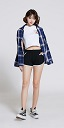
\includegraphics[]{ref4.jpg}}
    \quad
    \centering
    \subfloat[compare 1]{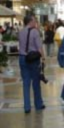
\includegraphics[]{compare1.png}}
    \quad
    \centering
    \subfloat[compare 2]{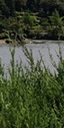
\includegraphics[]{compare2.png}}
    \caption{가설 검증을 위한 새 input 이미지}
\label{fig:newRefImg}
\end{figure}

\begin{figure}
    \begin{center}
        \fbox{\includegraphics[width = 0.6 \linewidth]{newRef-compABS.eps}}
        \caption{compare 1, 2와 new Ref.와의 HOG weight 차의 절대값 비교 그래프}
        \label{fig:newRefSubABSGraph}
    \end{center}
\end{figure}
그래프 Figure~\ref{fig:newRefSubABSGraph}를 보면, 눈으로 보기에도 파란색 점인 $|reference - compare1|$이 0에 가까워 보이며 실제로도 $|reference - compare1|<0.1$을 만족하는 값은 409개인 반면 $|reference - compare2|<0.1$을 만족하는 값은 224개에 불구하다. 전체값의 평균도 사람과 비교하였을때가 149, 풀과 비교하였을때가 219로 사람과 비교하였을 때의 값이 낮은것으로 나타났다.\\
위와같은 결과를 보아, 이번 코드는 HOG 알고리즘을 잘 구현하였으며, 기준이 되는 ref 이미지를 어떻게 잡는지도 중요하다는 것을 확인 하였다.

\end{document}